\section{解析と結果}

\subsection{チェレンコフ角の計算方法}
チャームバリオン分光実験におけるRICHの解析では、RICHの上流に置かれる飛跡検出器によって運動量ベクトルを得る。
その情報からチェレンコフリングの中心を計算し、光子の検出位置からチェレンコフ角を求める。
今回のシミュレーションでは、上流の飛跡検出器でリング中心を決定した後の状況を想定し、
入射する粒子の角度分布の$\sigma$は飛跡検出器の分解能$\SI{1}{mrad}$とした。
解析では、検出面の中心をリング中心とし、光子を検出した位置とリング中心との距離$r$をリングの半径と考え
リング半径と球面鏡の焦点距離$f$から$(\ref{eq:calcCherenkovAngleFromRadius})$式を用いてチェレンコフ角$\theta_{c}$を計算する。
その際に、光子を検出した位置は光子を検出したMPPCの中心として計算した。
各イベントで光子を検出したCH全ての平均の角度を、そのイベントでのチェレンコフ角とした。
また今回は実験データの解析と揃えるため、1つのMPPCに複数の光子が入った場合でも1回分として計算した。
\begin{equation}
  \theta_{c} = \arctan{\left(\frac{r}{f}\right)}
  \label{eq:calcCherenkovAngleFromRadius}
\end{equation}

\subsection{Dark currentなしでの評価}
まず、Dark currentを考慮しない解析を行った。
図\ref{fig:hitpattern1}に$\SI{2}{GeV/c}$の$\pi$が1つ入射した際のヒットパターンを示す。
チェレンコフリングがはっきりと確認できる。
リングから少し外れた位置で検出されているのはエアロゲルで散乱された光が偶然検出されたものである。
\begin{figure}[htbp]
  \centering
  \includegraphics[width=15cm, page=9]{images/chapter4/hitpattern2000MeV_pi.pdf}
  \caption{
    $\SI{2}{GeV/c}$の$\pi$が1つ入射した際のヒットパターン。
    チェレンコフリングがはっきり確認できる。
  }
  \label{fig:hitpattern1}
\end{figure}
次に、\ref{eq:calcCherenkovAngleFromRadius}式から計算したチェレンコフ角の分布を図\ref{fig:cherenkovAngleDistribution1}、\ref{fig:cherenkovAngleDistribution2}示す。
pは$\SI{3.4}{GeV/c}$まではチェレンコフ放射を起こさないため、$\SI{2.0}{GeV/c}$では$\pi$とKの分布のみとなっており、
$\pi$とKはよく分離できている。
しかし運動量が上がりリングサイズが大きくなってくると分布は近づいていき、
$\SI{6.0}{GeV/c}$では$\pi$とKの分布は重なっている。
また、各粒子に見られるテール部分は散乱光の影響によるもので、図に示す様に、エアロゲルでの散乱をなくした場合は
テールがなくなっていることが分かる。
\begin{figure}[htbp]
  \centering
  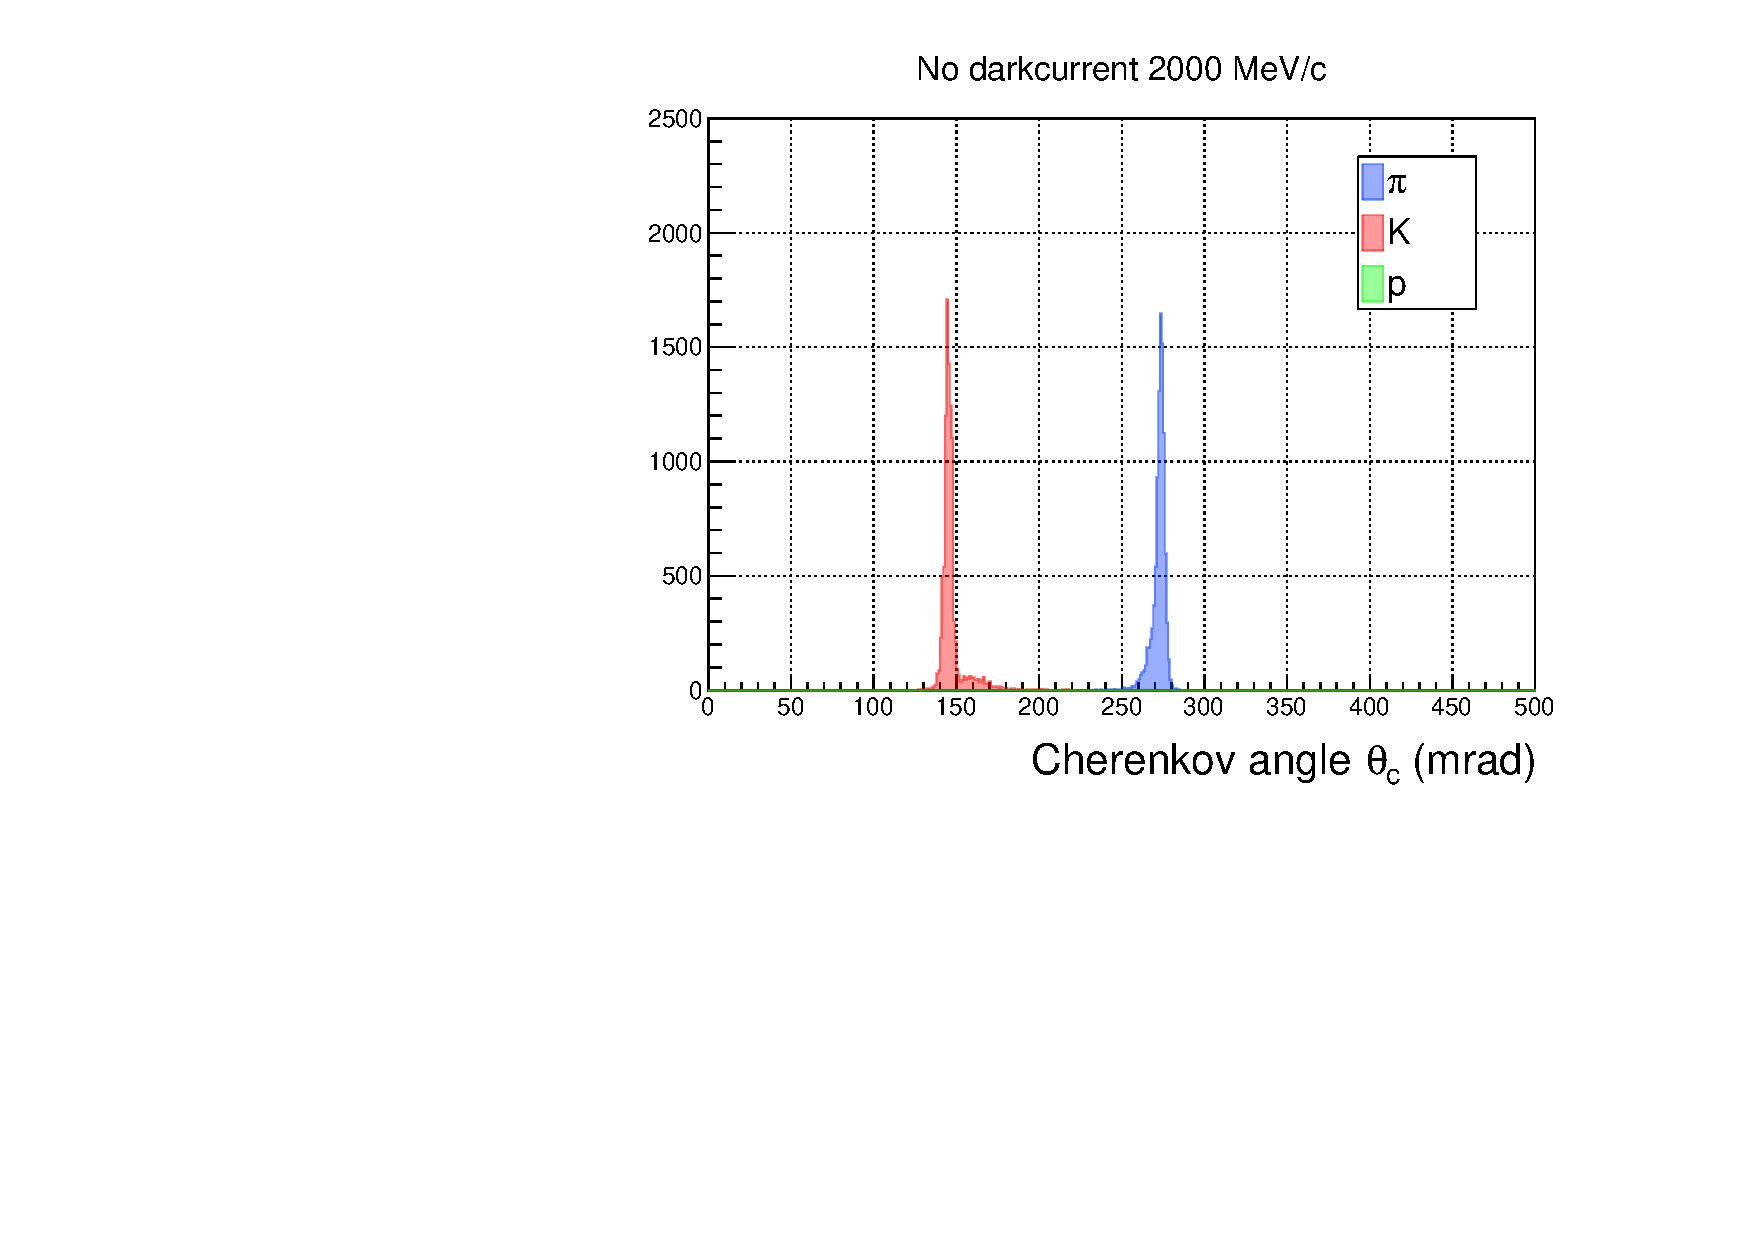
\includegraphics[width=15cm, page=1]{images/chapter4/2000MeV.pdf}
  \caption{
    $\SI{2.0}{GeV/c}$の時の各粒子のチェレンコフ角分布。青が$\pi$、赤がKの分布を表す。
    pは$\SI{3.4}{GeV/c}$以上でチェレンコフ放射を起こすため、$\pi$、Kの分布のみとなっている。
  }
  \label{fig:cherenkovAngleDistribution1}
\end{figure}
\begin{figure}[htbp]
  \centering
  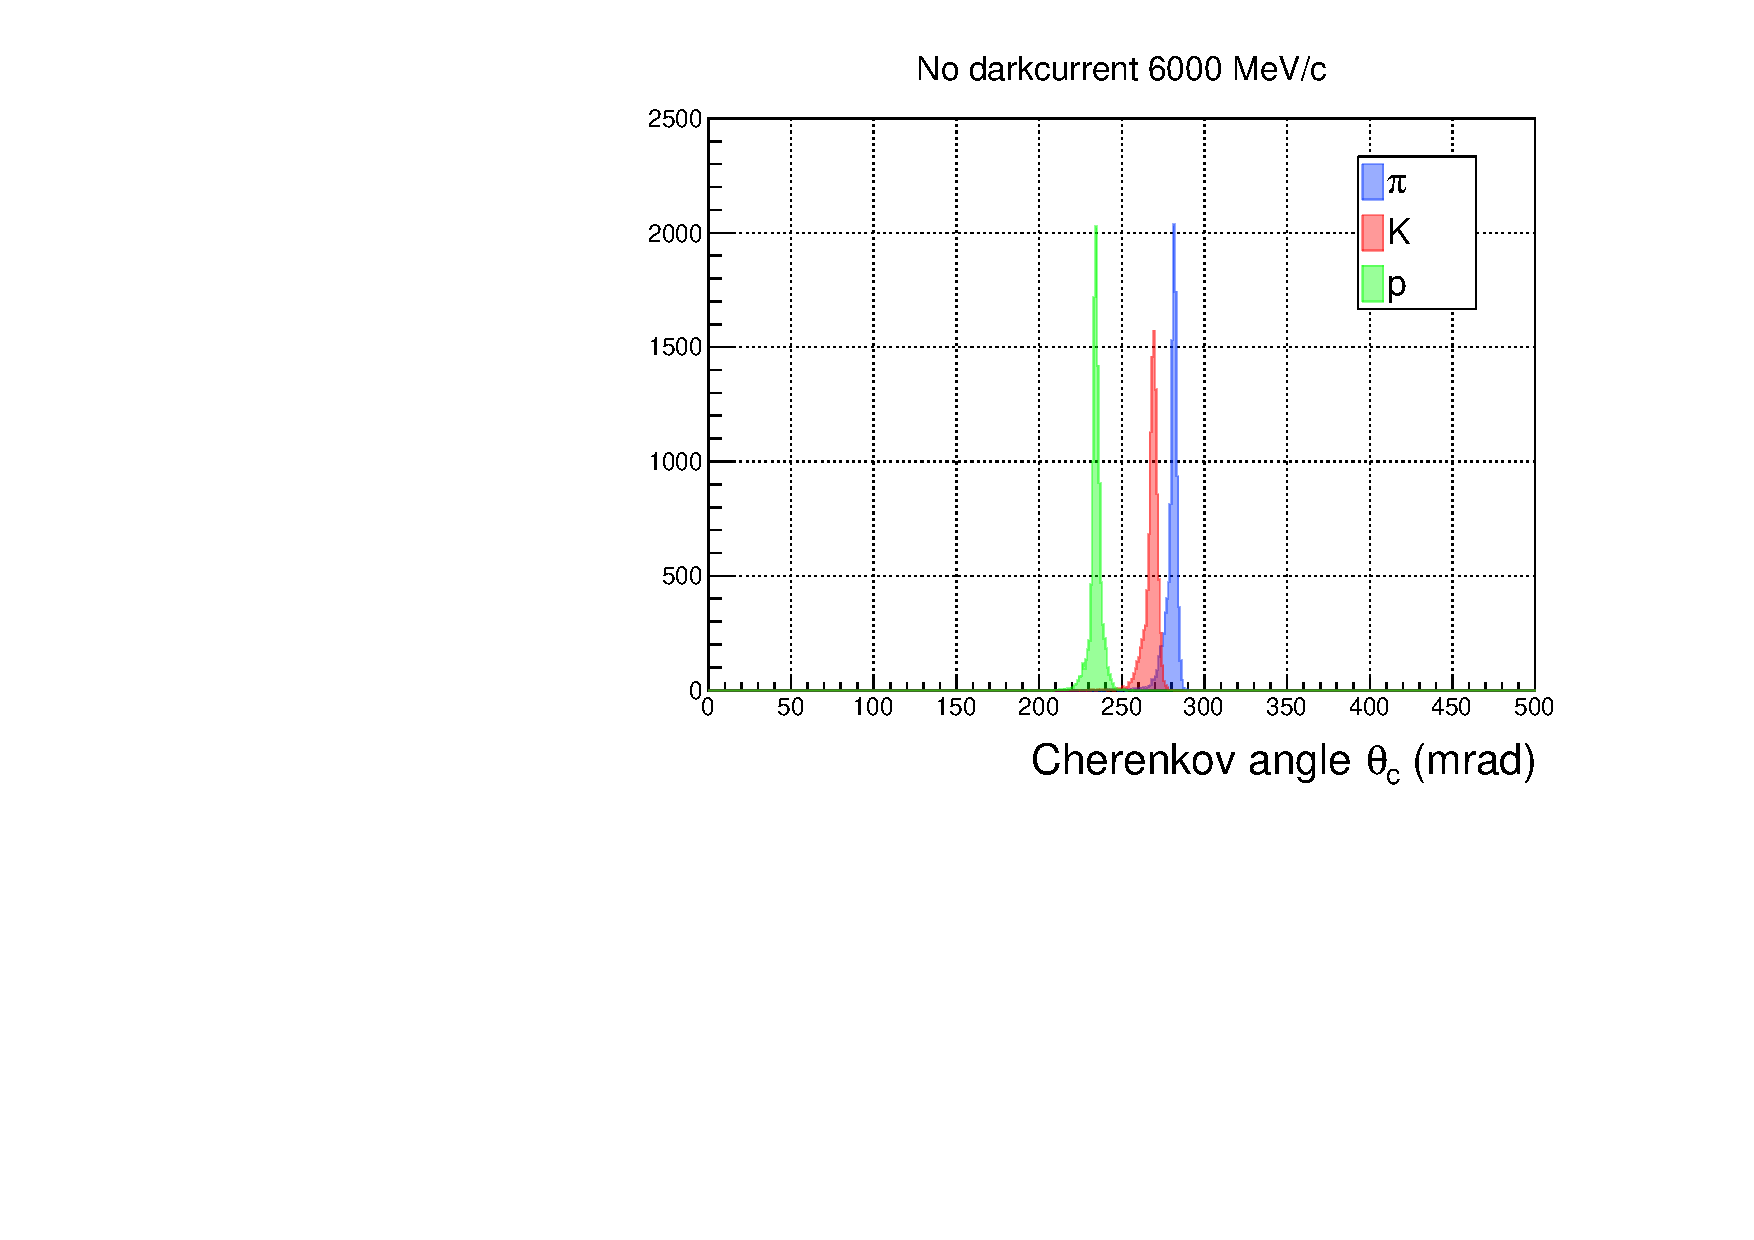
\includegraphics[width=15cm, page=1]{images/chapter4/6000MeV.pdf}
  \caption{
    $\SI{10.0}{GeV/c}$の時の各粒子のチェレンコフ角分布。青が$\pi$、赤がK、緑がpの分布を表す。
  }
  \label{fig:cherenkovAngleDistribution2}
\end{figure}

\begin{figure}[htbp]
  \centering
  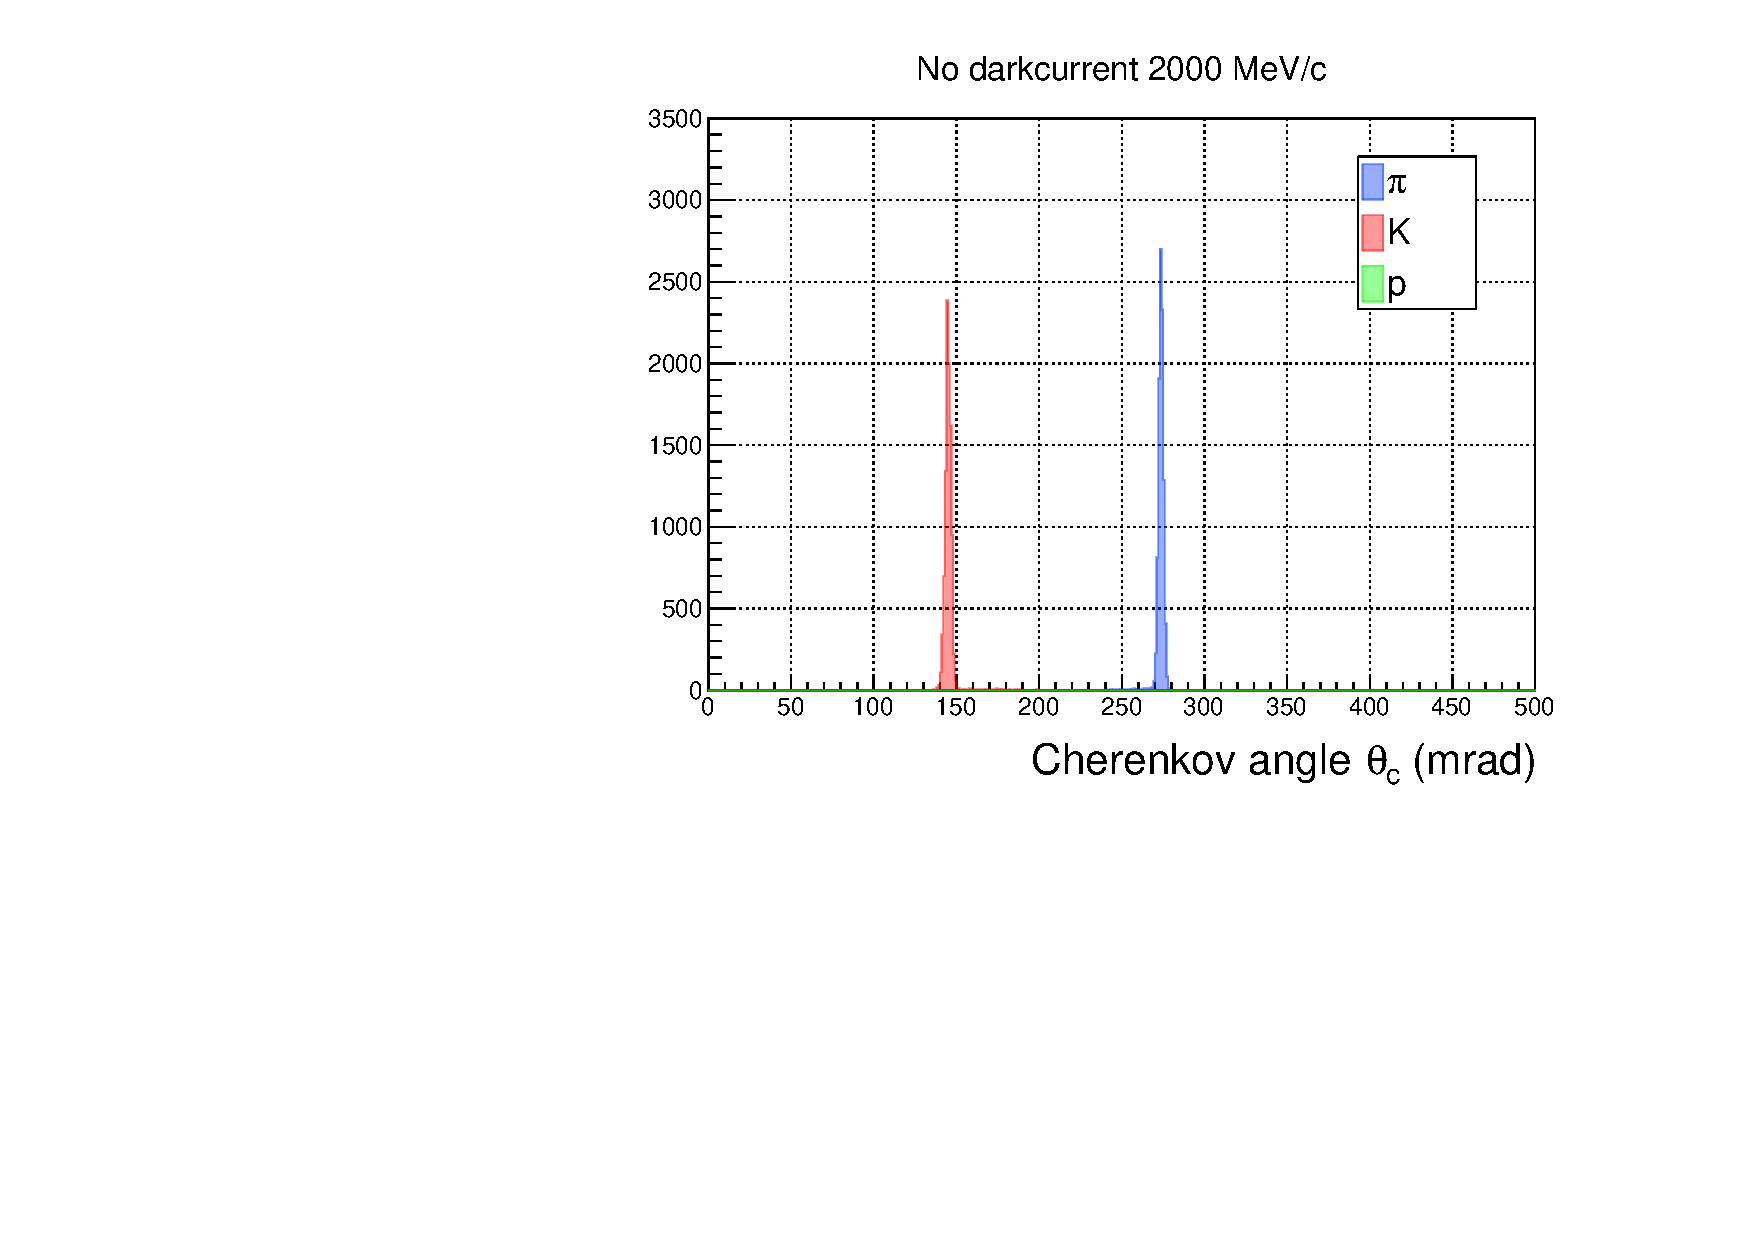
\includegraphics[width=15cm, page=1]{images/chapter4/2000MeV_noscatter.pdf}
  \caption{
  エアロゲルでの散乱をなくした場合の$\SI{2.0}{GeV/c}$でのチェレンコフ角分布。
  テールがなくなっていることがわかる。
  }
  \label{fig:cherenkovAngleDistribution3}
\end{figure}
図\ref{fig:angleMultiGraph1}に運動量に対するチェレンコフ角の分布を示す。
各粒子の角運動量でのチェレンコフ角分布をガウスフィットし、その際に得られたMeanとチェレンコフ角、Sigmaをエラーバーとして
プロットしている。
\begin{figure}[htbp]
  \centering
  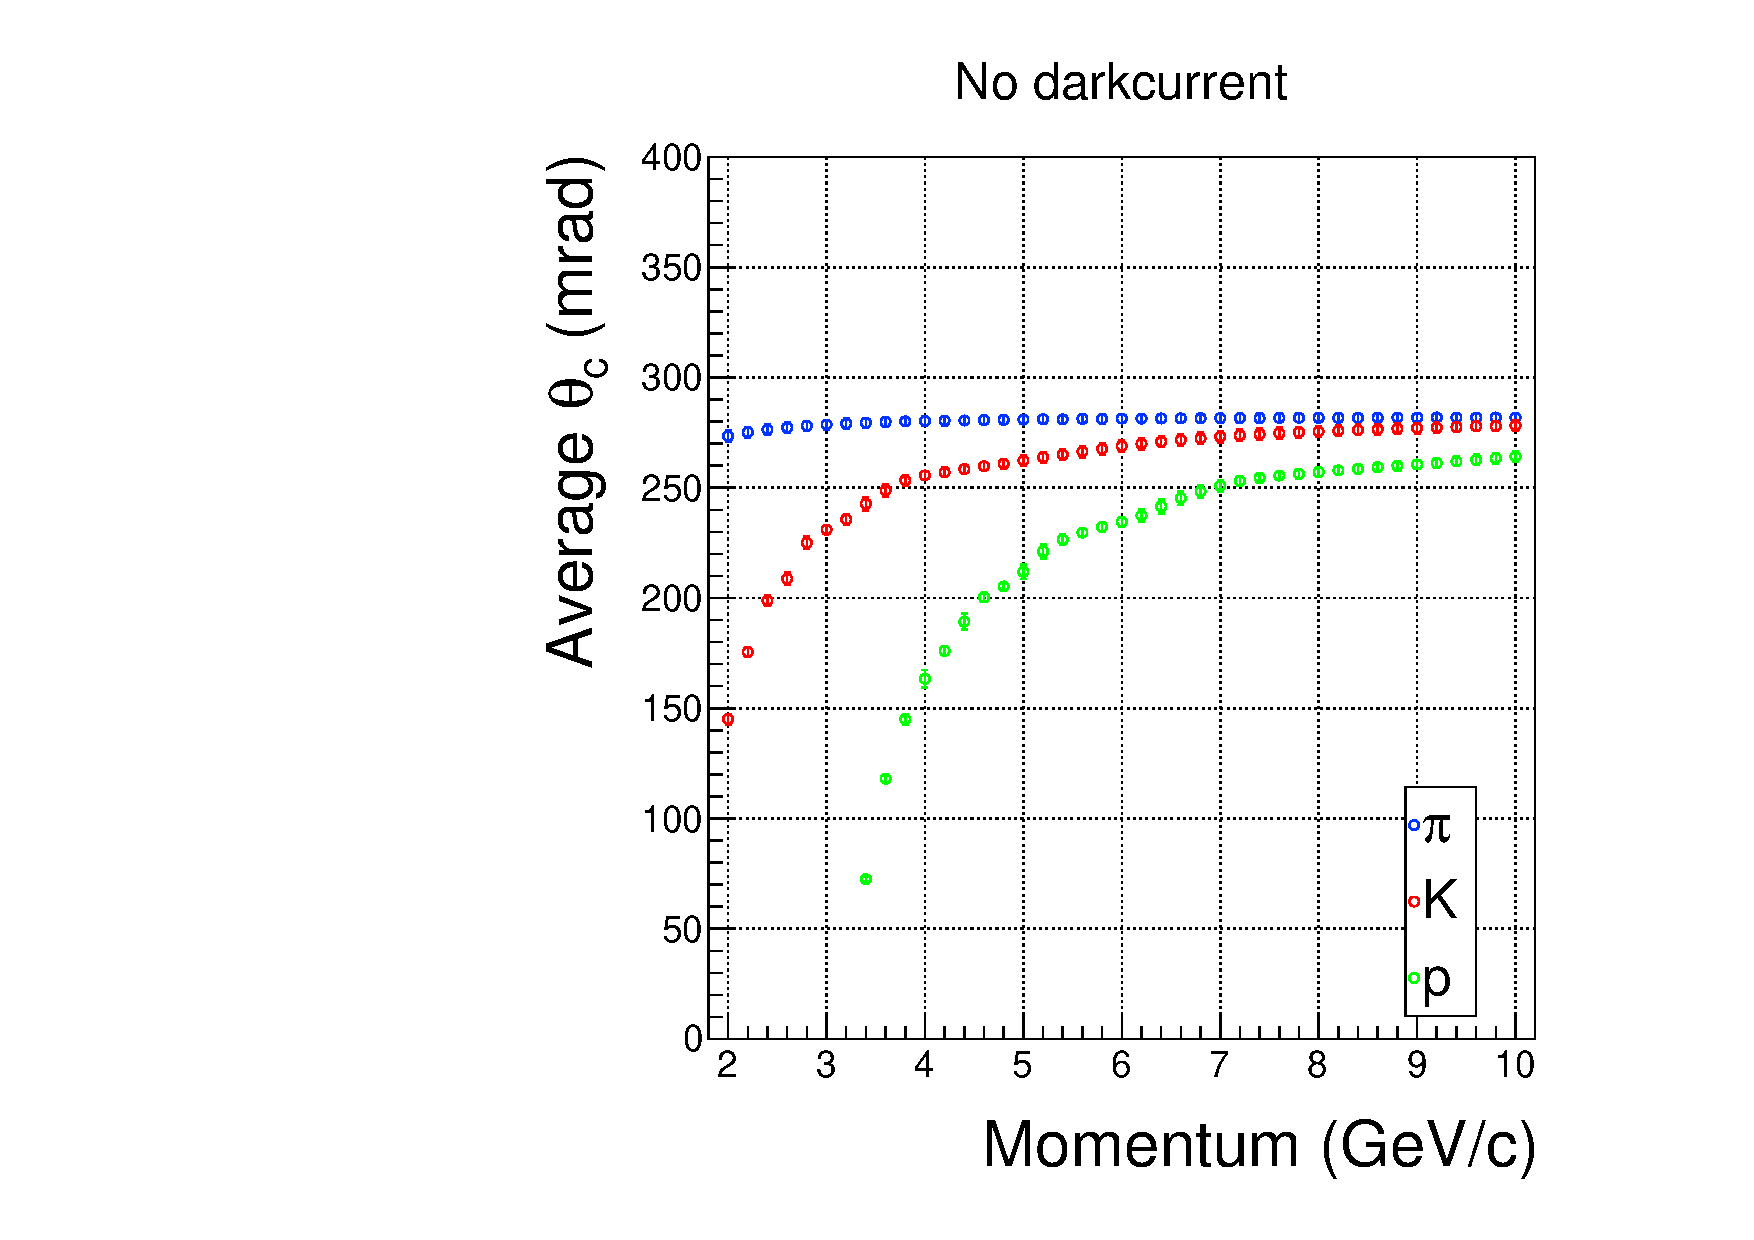
\includegraphics[width=15cm,page=1]{images/chapter4/angleAndMultiGraph.pdf}
  \caption{
    Dark currentを考慮しない場合の運動量毎のチェレンコフ角分布。青い点が$\pi$、赤い点がK、緑の点がpを示す。
    エラーバーはチェレンコフ角の分布をガウスフィットした際の$1\sigma$(角度分解能)としている。
  }
  \label{fig:angleMultiGraph1}
\end{figure}
また、各粒子の分布がどれだけ分離できているかを表すため、分離度の計算を行った。
各粒子のチェレンコフ角分布に対してガウスフィットを行い、チェレンコフ角分布のMeanとSigmaを求め、
粒子$i$、$j$それぞれのチェレンコフ角のMeanを$\theta_{i}$、$\theta_{j}$、Sigmaを$\sigma_{i}$、$\sigma_{j}$
とした時、粒子$i/j$の分離度$x_{ij}$を式\ref{eq:degreeOfSeparation}で計算した。
\begin{equation}
  x_{ij} = \frac{\left|\theta_{i} - \theta_{j}\right|}{\sigma_{i} + \sigma_{j}}
  \label{eq:degreeOfSeparation}
\end{equation}
その結果を図\ref{fig:angleMultiGraph3}に示す。
帝運動754

\begin{figure}[htbp]
  \centering
  \includegraphics[width=15cm,page=29]{images/chapter4/angleAndMultiGraph.pdf}
  \caption{
    Dark currentを考慮しない場合の分離度。
    縦軸は分離度$x$でログスケールとなっている。
    青の点が$\pi$/K、赤の点がK/p、緑の点がp/$\pi$の分離度を表す。
    Dark currentなしだと、2$-$6\space$\si{GeV/c}$の$\pi$/K、2$-$10\space$\si{GeV/c}$のK/pどちらも$3\sigma$以上分離できている。
  }
  \label{fig:angleMultiGraph3}
\end{figure}

\begin{figure}[htbp]
  \centering
  \includegraphics[width=15cm,page=2]{images/chapter4/angleAndMultiGraph.pdf}
  \caption{
    Dark currentを考慮した場合の運動量毎のチェレンコフ角分布。青い点が$\pi$、赤い点がK、緑の点がpを示す。
    エラーバーはチェレンコフ角の分布をガウスフィットした際の$1\sigma$(角度分解能)としている。
  }
  \label{fig:angleMultiGraph2}
\end{figure}

\begin{figure}[htbp]
  \centering
  \includegraphics[width=15cm,page=30]{images/chapter4/angleAndMultiGraph.pdf}
  \caption{
    Dark currentを考慮した場合の分離度。青の点が$\pi$/K、赤の点がK/p、緑の点がp/$\pi$の分離度を表す。
    Dark currentありだと、ほとんどの運動量領域において$2\sigma$以上分離できていない。
  }
  \label{fig:angleMultiGraph4}
\end{figure}